\chapter{Beschreibung Domain Layer Interfaces}

In diesem Kapitel werden die Interfaces des Domain Layers beschrieben.
Diese Interfaces liegen quasi auf dem "`Use Case"' Ring der Clean Architecture und kapseln die

\section{Repository}
\subsubsection{Repository Entwurfsmuster}
Es dient als Schnittstelle zwischen der Domänenschicht und der Datenzugriffsschicht. Es ist insbesondere in den Situationen hilfreich, in denen es viele unterschiedliche Domänenklassen oder viele unterschiedliche Zugriffe auf die Datenzugriffsschicht gibt.


Die Repository-Interfaces enthalten die Methodenköpfe der Repository-Methoden, jedoch keine Implementierung dieser.
Zu jedem Interface des Repositorys gibt es eine Klasse, die dieses Implementiert. Da das Repository ein Einzelstück ist (es soll ja die "`Single Source of Truth"' zwischen der inneren Schicht und den Datenquellen sein), gibt es nur ein Package, an Klassen, die die Methoden der Interfaces implementieren. 
Die Abstraktion ist in diesem Falle im Grunde nur zur Kapselung nötig.


Das Repository-Interface enthält die Methodenköpfe der Repository-Methoden. 
 
\section{Authentifizierung}

\begin{figure}[H]
\centering
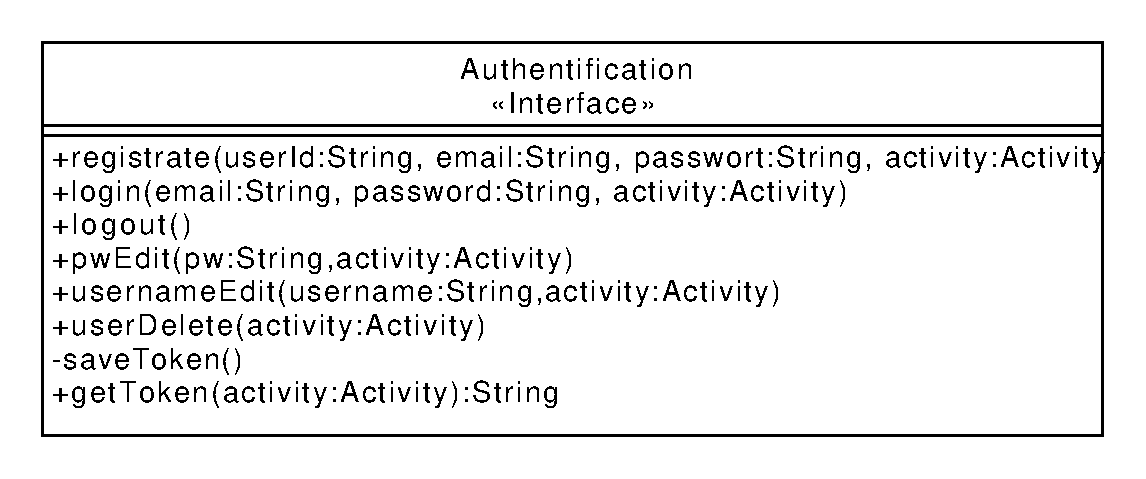
\includegraphics[width=0.7\textwidth]{generatedpics/Authentification_Search_Shopping.pdf}%
\caption{Authentification Schnittstelle}%
\label{appcomp}%
\end{figure}


Das Authentifizierugs-Interface definiert Methoden, die zur Authentifizierung eines Nutzers nötig sind. Dieses Interface wird dann von Klassen, die eine Authentifizierungsschnittstelle definieren, implementiert. Im Fall von Exzellenzkoch ist diese Klasse dann eine, die die Methoden von Firebase in den vordefinierten Interface-Methoden aufruft.

\section{ImportExport}

Im ImportExport-Interface stehen die nötigen Methodenvorgaben, die die Intents brauchen: 
\begin{lstlisting}
importExport.shareRecipe(Recipe) : void
importExport.parseIntent(Intent) : privateRecipe
\end{lstlisting}